% Provenance (never printed): see sources/outline_sources.md (Year 3:
% dislocation and diffusion creep; flow laws; deformation maps; shear zones and
% kinematic indicators). Brief: sources/book5/BRIEFS.md, ch. 7. Curves from
% figdata/bachelor-3/flow_laws.py. Exercise and problem values in the Book 5
% scratch calculator calc/ch07.py.
\chapter{آليات التشوّه ونطاقات القصّ}\label{ch:b3:deformation-mechanisms}

عند السطح، يتحطّم الغرانيت في الجبال على طول الصدوع. على عمق عشرين
كيلومترًا، يتدفّق الغرانيت نفسه كالتوفي في نطاق قصّ عرضه بضع
مئات الأمتار، فتتدحرج فلسباراته لتصير عيونًا، ويُمطّ كوارتزه
إلى شرائط. ويمكن للبلّورة أن تنساب دون أن تنكسر لأنها ليست كاملة أبدًا:
تتحرّك بعيوبها، صفًّا واحدًا من الذرات في كلّ مرّة، أو بانتشار الذرات من
أحد أوجه الحبيبة إلى الوجه الآخر. يتتبّع هذا الفصل تلك الآليات من
الشبكة البلّورية إلى القوانين التي تستخدمها الجيوديناميكا، وإلى الخرائط التي تبيّن أيّ
آلية تغلب، وإلى نطاقات القصّ التي تسجّل فيها الصخرة كيفية حركتها.

\begin{recall}
تُعرض العيوب النقطية وقانون أرينيوس وطاقة التنشيط في مجلّدات
كتب الكيمياء الجامعية؛ ومعامل الانتشار في كتب الفيزياء.
الإجهاد والانفعال، والقطع الناقص للانفعال، والقصّ البسيط وقطعه الناقص
($S_{1,2} = \sqrt{1 + \gamma^2/4} \pm \gamma/2$، والمحور الأطول عند $\theta'$ من
\omterm{def:b3:deformation-mechanisms:kinematic}{اتجاه القصّ} مع $\tan2\theta' = 2/\gamma$)، والزحف وفق قانون القوّة بثوابته
لكوارتزيت مبلَّل والأوليفين الجاف، ومغلّف المتانة
وانتقال الهشاشة--اللدونة موجودان في مجلد السنة الأولى، في فصله عن
الإجهاد والانفعال والريولوجيا؛ والتورّق والتخطّط والميلونيت الوصفي
في فصله عن الصدوع والطيات والنسُج. وترد اللزوجة الفعّالة
للوشاح في \cref{ch:b3:mantle-convection}.
\end{recall}

\section{عيوب البلّورات}

لقصّ بلّورة كاملة، كان يجب أن تنكسر كلّ رابطة عبر مستوى شبكي
في آن واحد، ويتطلّب ذلك إجهادًا من رتبة عُشر
معامل القصّ، وهو في الوشاح نحو \qty{8e10}{Pa}
(\cref{ch:b3:mantle-convection}): آلاف الميغاباسكال. أما البلّورات الحقيقية
فتخضع عند إجهادات أدنى بكثير، لأنها تنزلق صفًّا واحدًا من الذرات في كلّ مرّة.

\begin{definition}[الانخلاع]\label{def:b3:deformation-mechanisms:dislocation}
\emph{الانخلاع}\index{الانخلاع (عيب بلّوري)} عيب خطّي في
البلّورة: الحدّ الفاصل داخل البلّورة بين جزء من مستوى شبكي
قد انزلق وجزء لم ينزلق. ومتجهة \emph{برغرز}
$\mathbf b$ هي الانزلاق الذي تحمله، بمقدار تباعد شبكي واحد في اتجاه
شبكي. وفي الانخلاع الحافّي تكون $\mathbf b$ عمودية على الخطّ،
وهو حافّة نصف مستوٍ إضافي من الذرات؛ وفي الانخلاع اللولبي تكون
موازية للخطّ. ويتحرّك الانخلاع \emph{بالانزلاق} على مستوى انزلاقه،
ويخرج الانخلاع الحافّي من ذلك المستوى \emph{بالتسلّق}، إذ تنتشر ذرات أو
فجوات إلى حافّة نصف مستواه أو منها.
\end{definition}

\begin{omfigure}
\begin{tikzpicture}[font=\scriptsize, x=0.42cm, y=0.42cm]
% (a) lower half: 10 columns; upper half: 11 columns squeezed over the same width
\foreach \j in {0,...,3} {\foreach \i in {0,...,9} {\fill[gray!70] (\i,\j) circle (0.13);}}
\foreach \j/\s in {4/0.9, 5/0.92, 6/0.94, 7/0.96} {\foreach \i in {0,...,10} {
  \pgfmathsetmacro{\x}{(\i-5)*\s + 4.5}
  \ifnum\i=5 \fill[red!70!black] (\x,\j) circle (0.15); \else \fill[gray!70] (\x,\j) circle (0.13); \fi}}
\draw[thick, blue!60!black] (-0.6,3.5) -- (9.6,3.5);
\node[anchor=east, blue!60!black] at (-0.7,3.5) {مستوى الانزلاق};
\draw[red!70!black, very thick] (4.1,3.62) -- (4.9,3.62) (4.5,3.62) -- (4.5,4.2);
\node[red!70!black] at (4.5,8.2) {نصف مستوى إضافي};
\draw[->, thick] (1.0,9.2) -- (3.0,9.2) node[right] {$\tau$};
\draw[<-, thick] (6.0,-1.0) -- (8.0,-1.0) node[right] {$\tau$};
% (b) after glide: the upper half shifted by one spacing
\begin{scope}[shift={(14,0)}]
\foreach \j in {0,...,3} {\foreach \i in {0,...,9} {\fill[gray!70] (\i,\j) circle (0.13);}}
\foreach \j in {4,...,7} {\foreach \i in {1,...,10} {\fill[gray!70] (\i,\j) circle (0.13);}}
\draw[thick, blue!60!black] (-0.6,3.5) -- (10.6,3.5);
\draw[|<->|] (9,8.3) -- (10,8.3) node[midway, above] {$\mathbf b$};
\end{scope}
\node[anchor=north] at (4.5,-1.8) {\foreignlanguage{arabic}{(أ) انخلاع حافّي}};
\node[anchor=north] at (19,-1.8) {\foreignlanguage{arabic}{(ب) بعد أن انزلق خارجًا}};
\end{tikzpicture}

\par\smallskip{\small (أ) انخلاع حافّي: نصف مستوى إضافي من الذرات (باللون الأحمر)
ينتهي عند مستوى الانزلاق، فيشوّه الشبكة حول حافّته (الرمز
$\perp$). تحت إجهاد القصّ $\tau$ ينزلق على طول مستوى الانزلاق
بكسر صفّ واحد من الروابط في كلّ مرّة وإعادة تكوينه. (ب) عندما يعبر \omterm{def:b3:deformation-mechanisms:dislocation}{الانخلاع}
البلّورة، فقد انزلق النصف العلوي بمقدار متجهة برغرز $\mathbf b$، وعادت الشبكة
كاملة من جديد.}\label{fig:b3:deformation-mechanisms:dislocation}
\end{omfigure}

تقاوم الشبكة انزلاق \omterm{def:b3:deformation-mechanisms:dislocation}{الانخلاع} بإجهاد صغير، هو
إجهاد بيرلس، ويعتمد على قوّة الروابط واتجاهها:
ولهذا تكون بعض أنظمة الانزلاق في المعدن سهلة وبعضها صعبًا. ومع
تشوّه البلّورة تتكاثر الانخلاعات وتتشابك؛ فتعيق بعضها بعضًا،
وتتصلّب البلّورة، إلّا إذا استطاعت أن تتسلّق العوائق أو تفنى، وهذا
يتطلّب الانتشار، ومن ثَمّ الحرارة.

\section{آليات الزحف}

\begin{definition}[آليات الزحف]\label{def:b3:deformation-mechanisms:creep}
في \emph{الزحف الانخلاعي}\index{الزحف الانخلاعي} تتشوّه البلّورات بانزلاق
الانخلاعات، ويُحرّرها التسلّق من العوائق. وفي
\emph{الزحف الانتشاري}\index{الزحف الانتشاري} تغيّر البلّورات شكلها بانتشار الذرات،
عبر الشبكة (زحف نابارو--هيرينغ) أو على طول
حدود الحبيبات (زحف كوبل)، من الأوجه الواقعة تحت أعلى إجهاد عمودي
إلى الأوجه الواقعة تحت أدنى إجهاد. وفي \emph{انزلاق حدود الحبيبات}\index{انزلاق حدود الحبيبات}
تنزلق الحبيبات بعضها فوق بعض على طول حدودها، وتُغلق الفجوات
بالانتشار أو بالزحف الانخلاعي. وفي \emph{الإذابة
بالضغط}\index{الإذابة بالضغط} تذوب المادّة في غشاء سائل على الأوجه
الواقعة تحت إجهاد مرتفع، وتترسّب حيث يكون الإجهاد منخفضًا، أو تُنقل
بعيدًا.
\end{definition}

\begin{proposition}[اعتماد الزحف الانتشاري على حجم الحبيبات]\label{prop:b3:deformation-mechanisms:grain-size}
عند إجهاد منخفض $\sigma$، تزحف صخرة حجم حبيباتها $d$ بالانتشار بالمعدّل
\[
  \dot\varepsilon \approx B_L\frac{D_L\Omega}{k_BT}\frac{\sigma}{d^2}
  \quad\text{(عبر الشبكة)},\qquad
  \dot\varepsilon \approx B_B\frac{\delta D_B\Omega}{k_BT}\frac{\sigma}{d^3}
  \quad\text{(على طول الحدود)},
\]
حيث $D_L$ و$D_B$ معاملا الانتشار في الشبكة وفي
الحدود، و$\delta$ عرض الحدّ، و$\Omega$ حجم الذرة،
و$k_B$ ثابت بولتزمان، و$B_L$ و$B_B$ أعداد من رتبة العشرة تعتمد على
شكل الحبيبات.
\end{proposition}

\begin{proof}
يغيّر الإجهاد العمودي $\sigma$ على وجه ما الشغل اللازم لتكوين فجوة فيه
بمقدار $\sigma\Omega$، فيختلف تركيز الفجوات $C$ بين
الوجوه الواقعة تحت الشدّ والوجوه الواقعة تحت الضغط بمقدار $\Delta C \approx C\sigma\Omega/
(k_BT)$ حين $\sigma\Omega \ll k_BT$. وعبر مسافة من رتبة $d$، يكون
الدفق الانتشاري للفجوات، ومن ثَمّ للذرات في الاتجاه المعاكس، من رتبة $D\Delta
C/d$ لكل وحدة مساحة. عبر الشبكة يعبر الدفق مساحةً من رتبة
$d^2$، وعلى طول الحدود مساحةً من رتبة $\delta d$. الحجم المنقول لكل
وحدة زمن، مقسومًا على حجم الحبيبة $d^3$، هو معدّل الانفعال: من رتبة
$(D_L\sigma\Omega/k_BT)\,d^2/(d\cdot d^3) = D_L\sigma\Omega/(k_BTd^2)$ في
الشبكة، و$(D_B\sigma\Omega/k_BT)\,\delta d/(d\cdot d^3) = \delta D_B
\sigma\Omega/(k_BTd^3)$ على الحدود. حاصل الضرب $C\,D$ هو معامل
الانتشار الذاتي المكتوب $D$ في نصّ القضية.
\end{proof}

\omterm{def:b3:deformation-mechanisms:creep}{الزحف الانتشاري} خطّي بالنسبة إلى الإجهاد، وهو انسياب لزج حقيقي، وهو سريع في
الصخور دقيقة الحبيبات: إذ يجعل تنصيف حجم الحبيبات زحف كوبل أسرع ثماني مرات
(الشكل أدناه). ولا يعتمد \omterm{def:b3:deformation-mechanisms:creep}{الزحف الانخلاعي} على حجم الحبيبات، لكنه يتزايد
بأسّ مرتفع للإجهاد.

\begin{omfigure}
\begin{tikzpicture}[font=\scriptsize, x=1cm, y=1cm]
\foreach \cx/\lab in {0/{(أ) عبر الشبكة البلورية}, 6/{(ب) على طول الحدود}} {
  \begin{scope}[shift={(\cx,0)}]
  \draw[thick, fill=gray!10] (-1.6,-1.1) -- (-0.6,-1.7) -- (1.0,-1.6) -- (1.7,-0.4) -- (1.5,1.0) -- (0.4,1.7) -- (-1.2,1.3) -- (-1.8,0.2) -- cycle;
  \draw[->, very thick, red!70!black] (0,2.6) -- (0,1.9);
  \draw[->, very thick, red!70!black] (0,-2.6) -- (0,-1.9);
  \node[red!70!black] at (0.45,2.45) {$\sigma$};
  \draw[<-, very thick, gray] (2.7,0.3) -- (2.0,0.3);
  \draw[<-, very thick, gray] (-2.8,-0.3) -- (-2.1,-0.3);
  \node[anchor=north] at (0,-2.8) {\foreignlanguage{arabic}{\lab}};
  \end{scope}
}
\foreach \sx in {1,-1} {\foreach \y in {-0.5,0.5} {
  \draw[->, blue!60!black, thick] (0.15*\sx,1.25) .. controls (0.5*\sx,\y+0.6) and (0.9*\sx,\y+0.15) .. (1.45*\sx,\y);
  \draw[->, blue!60!black, thick] (0.15*\sx,-1.25) .. controls (0.5*\sx,\y-0.6) and (0.9*\sx,\y-0.15) .. (1.45*\sx,\y);
}}
\draw[->, blue!60!black, thick] (6.4,1.62) -- (7.45,1.05) -- (7.65,0.2);
\draw[->, blue!60!black, thick] (5.9,1.45) -- (4.85,1.35) -- (4.25,0.3);
\draw[->, blue!60!black, thick] (6.9,-1.62) -- (7.0,-1.6) -- (7.6,-0.6);
\draw[->, blue!60!black, thick] (5.6,-1.6) -- (5.4,-1.68) -- (4.45,-1.15) -- (4.25,-0.3);
\end{tikzpicture}

\par\smallskip{\small زحف انتشاري لحبيبة تقلّصت على طول $\sigma$. تنتقل الذرات
من الأوجه الواقعة تحت أعلى ضغط وتُضاف إلى الأوجه الواقعة تحت
أدنى ضغط (باللون الأزرق)، فتتسطّح الحبيبة وتستطيل (الأسهم الرمادية): (أ)
عبر داخل الحبيبة، زحف نابارو--هيرينغ؛ (ب) على طول حدودها،
زحف كوبل.}\label{fig:b3:deformation-mechanisms:diffusion}
\end{omfigure}

تُصلح البلورات المشوَّهة نفسها أيضًا أثناء تشوّهها.

\begin{definition}[الاستعادة، الحبيبات الفرعية، إعادة التبلور الديناميكية]\label{def:b3:deformation-mechanisms:recrystallisation}
\emph{الاستعادة}\index{الاستعادة (لدونة البلورات)} هي إعادة ترتيب
الانخلاعات بالتسلّق والانزلاق المتقاطع إلى تراكيب أدنى طاقةً،
وتلاشيها. وتقسّم الانخلاعات المرتّبة في جدران الحبيبةَ إلى
\emph{الحبيبات الفرعية}\index{الحبيبات الفرعية}، أجزاء من الحبيبة تميل شبكاتها
بمقدار بضع درجات بعضها عن بعض. \emph{إعادة
التبلور الديناميكية}\index{إعادة التبلور الديناميكية} هي استبدال الحبيبات المتشوّهة، أثناء
التشوّه، بحبيبات جديدة أقلّ انخلاعًا، إمّا
بدوران الحبيبات الفرعية حتى تصير حبيبات، أو بهجرة
حدود الحبيبات إلى الجيران الأكثر تشوّهًا.
\end{definition}

\begin{definition}[التوجّه البلوري المفضَّل]\label{def:b3:deformation-mechanisms:cpo}
يمتلك الصخرُ \emph{التوجّه البلوري المفضَّل}\index{التوجّه البلوري المفضَّل}
(CPO) حين لا تكون شبكات حبيباته موجَّهةً
عشوائيًا، بل تتجمّع حول اتجاهات يحدّدها التشوّه؛ ويُنتجه \omterm{def:b3:deformation-mechanisms:creep}{الزحف الانخلاعي}
بتدوير منظومات الانزلاق في كل حبيبة نحو اتجاه الانسياب.
\end{definition}

يرث الصخرُ ذو \omterm{def:b3:deformation-mechanisms:cpo}{التوجّه البلوري المفضَّل} لاتناحيةَ بلوراته: فسرعاتُ الموجات الزلزالية فيه،
مثلًا، تتوقّف على الاتجاه، وهذا ما يتيح لعلم الزلازل أن يرى نسيجَ
الوشاحِ العميق. أمّا \omterm{def:b3:deformation-mechanisms:creep}{الزحف الانتشاري} \omterm{def:b3:deformation-mechanisms:creep}{وانزلاق حدود الحبيبات}، اللذان يتيحان
للحبيبات أن تدور بحرّية، فلا يُنشئانه.

\section{قوانين الانسياب}

\begin{definition}[قانون الانسياب، أسّ الإجهاد، درجة الحرارة المتجانسة]\label{def:b3:deformation-mechanisms:flow-law}
يُعطي \emph{قانون الانسياب}\index{قانون الانسياب} معدّلَ الانفعال لصخرٍ يتشوّه
بآلية واحدة، دالّةً للإجهاد التفاضلي $\sigma$ وحجم الحبيبات
$d$، ودرجة الحرارة $T$ والضغط $P$:
\[
  \dot\varepsilon = A\,\sigma^nd^{-m}\exp\Bigl(-\frac{E + PV}{RT}\Bigr),
\]
حيث $A$، $n$، $m$، وطاقةُ التنشيط $E$، وحجمُ التنشيط $V$
تُقاس في المختبر. \emph{أسّ الإجهاد}\index{أسّ الإجهاد} هو $n$،
وأسّ حجم الحبيبات $m$. \emph{درجة الحرارة
المتجانسة}\index{درجة الحرارة المتجانسة} لمعدنٍ هي $T/T_m$، وهي
درجته المطلقة على درجة حرارة انصهاره المطلقة.
\end{definition}

في القوانين المستعملة هنا، يكون للزحف الانخلاعي $n$ قدرُه 3.5 أو 4 و$m = 0$؛
وللزحف الانتشاري $n = 1$ و$m = 2$ أو 3 (انظر \cref{prop:b3:deformation-mechanisms:grain-size}).
يزداد الزحف كلّما اقتربت \omterm{def:b3:deformation-mechanisms:flow-law}{درجة الحرارة المتجانسة} من 1. ينصهر الفورستيريت عند \qty{1890}{\celsius}، فيكون الوشاح عند \qty{1300}{\celsius}
تبلغ $T/T_m = 0.73$؛ أمّا الجليد عند \qty{-10}{\celsius} فيبلغ 0.96، ولهذا السبب
تنساب الأنهار الجليدية. وقيم الأوليفين المعتمدة هنا هي تلك الواردة في
مجموعة مخبرية واسعة الاستعمال: الأوليفين الجاف في \omterm{def:b3:deformation-mechanisms:creep}{الزحف الانخلاعي}، $A =
\num{1.1e5}$، $n = 3.5$، $E = \qty{530}{kJ.mol^{-1}}$، $V =
\qty{14}{cm^3.mol^{-1}}$؛ وفي \omterm{def:b3:deformation-mechanisms:creep}{الزحف الانتشاري}، $A = 10^{9.2}$، $n = 1$، $m = 3$،
$E = \qty{375}{kJ.mol^{-1}}$، $V = \qty{5}{cm^3.mol^{-1}}$ (الإجهاد بوحدة ميغاباسكال،
حجم الحبيبات بالميكرومترات، والزمن بالثواني)؛ أمّا قيم الكوارتزيت الرطب فمأخوذة من
مجلد السنة الأولى. يُضعف الماء الأوليفين: عند فوغاسيتية مائية تقارب
\qty{300}{MPa}، تزحف تجمّعات الأوليفين أسرع من الجافة بخمس إلى ست مرات
في \omterm{def:b3:deformation-mechanisms:creep}{الزحف الانخلاعي}، وأسرع بخمس مرات في \omterm{def:b3:deformation-mechanisms:creep}{الزحف الانتشاري}.
% ledger: bowen14:mgo-sio2, azuma17:olivine, lopez:flow-laws, codata:R, mk00:diffusion, mk00:dislocation

\begin{proposition}[اللزوجة الفعّالة]\label{prop:b3:deformation-mechanisms:viscosity}
للصخر الخاضع \omterm{def:b3:deformation-mechanisms:flow-law}{لقانون الانسياب} $\dot\varepsilon = A'\sigma^n$ عند قيم معلومة من $T$ و$P$
و$d$ له اللزوجة الفعّالة
\[
  \eta_{\mathrm{eff}} = \frac{\sigma}{2\dot\varepsilon}
  = \tfrac12A'^{-1/n}\,\dot\varepsilon^{(1-n)/n}:
\]
من أجل $n > 1$ تنخفض اللزوجة كلّما تشوّه الصخر أسرع.
\end{proposition}

\begin{proof}
لمائعٍ نيوتونيّ، يكون $\sigma = 2\eta\dot\varepsilon$ في الجريان أحادي المحور، وفق تعريف اللزوجة؛
$\eta_{\mathrm{eff}}$ هي لزوجة المائع النيوتوني
الذي يجري بالمعدّل نفسه تحت الإجهاد نفسه. بتعويض
$\sigma = (\dot\varepsilon/A')^{1/n}$ نحصل على الصيغة الثانية.
\end{proof}

يحتاج الكوارتزيت الرطب عند \qty{400}{\celsius} الجاري بمعدّل \qty{e-14}{s^{-1}} إلى
\qty{65}{MPa} وله لزوجة فعّالة مقدارها \qty{3.3e21}{Pa.s}؛ عند
\qty{500}{\celsius}، \qty{18}{MPa} و\qty{9e20}{Pa.s}: مئةُ درجةٍ تقسم القوّةَ
على أكثر من ثلاثة (انظر الشكل أدناه). الأوليفين الجاف عند
\qty{1100}{\celsius} و\qty{1}{GPa} يحتاج إلى \qty{3}{MPa} فقط. تُبنى مغلّفات القوّة
في مجلد السنة الأولى انطلاقًا من هذه القوانين بعينها.

\begin{omfigure}
\begin{tikzpicture}
\begin{groupplot}[group style={group size=2 by 1, horizontal sep=1.6cm},
  omrecord, width=0.47\linewidth, height=0.47\linewidth, xmode=log,
  xmin=1, xmax=1000, ymin=-20, ymax=-6, xlabel={الإجهاد التفاضلي \babelsublr{(MPa)}},
  legend style={font=\scriptsize, at={(0.97,0.03)}, anchor=south east, legend columns=1}]
\nextgroupplot[ylabel={\mbox{\textdir TLT $\log_{10}\dot\varepsilon$ (\unit{s^{-1}})}}, title={(أ) الكوارتزيت الرطب},
  title style={font=\small}]
% computed in figdata/bachelor-3/flow_laws.py; ledger: lopez:flow-laws, azuma17:olivine
\addplot[omDef, thick] table[x=s, y=r600] {figdata/out/bachelor-3-flow_laws-quartz.dat};
\addlegendentry{\qty{600}{\celsius}}
\addplot[red!70!black, thick, densely dashed] table[x=s, y=r500] {figdata/out/bachelor-3-flow_laws-quartz.dat};
\addlegendentry{\qty{500}{\celsius}}
\addplot[black, thick, densely dotted] table[x=s, y=r400] {figdata/out/bachelor-3-flow_laws-quartz.dat};
\addlegendentry{\qty{400}{\celsius}}
\draw[gray] (axis cs:1,-14) -- (axis cs:1000,-14);
\nextgroupplot[title={(ب) الأوليفين الجاف، \mbox{\textdir TLT \qty{1}{GPa}}}, title style={font=\small}]
\addplot[omDef, thick] table[x=s, y=r1300] {figdata/out/bachelor-3-flow_laws-olivine.dat};
\addlegendentry{\qty{1300}{\celsius}}
\addplot[red!70!black, thick, densely dashed] table[x=s, y=r1100] {figdata/out/bachelor-3-flow_laws-olivine.dat};
\addlegendentry{\qty{1100}{\celsius}}
\addplot[black, thick, densely dotted] table[x=s, y=r900] {figdata/out/bachelor-3-flow_laws-olivine.dat};
\addlegendentry{\qty{900}{\celsius}}
\draw[gray] (axis cs:1,-14) -- (axis cs:1000,-14);
\end{groupplot}
\end{tikzpicture}

\par\smallskip{\small قوانين الانسياب للزحف الانخلاعي: معدّل الانفعال بدلالة الإجهاد عند
ثلاث درجات حرارة. ميل المنحنى على هذه المحاور هو \omterm{def:b3:deformation-mechanisms:flow-law}{أسّ الإجهاد}، 4 للكوارتزيت
و3.5 للأوليفين؛ يمثّل الخطّ الرمادي معدّلًا جيولوجيًّا للانفعال،
\qty{e-14}{s^{-1}}. يحتاج الأوليفين إلى درجات حرارة أعلى بنحو \qty{600}{\celsius}
من الكوارتز كي يجري بالسهولة نفسها.}\label{fig:b3:deformation-mechanisms:flow-laws}
\end{omfigure}

\section{خرائط آليات التشوّه}

تعمل عدّة آليات بالتوازي، ويحمل الأسرع منها التشوّه.

\begin{definition}[خريطة آليات التشوّه]\label{def:b3:deformation-mechanisms:deformation-map}
\emph{خريطة آليات التشوّه}\index{خريطة آليات التشوّه} لمعدن أو صخر
تُظهر، على محورين من المتغيّرات الإجهاد وحجم الحبيبات ودرجة الحرارة،
المناطقَ التي تكون فيها كلُّ آليةٍ هي الأسرعَ، مع خطوط كنتورية
لمعدّل الانفعال الكلّي.
\end{definition}

\begin{proposition}[حدّ الآليات]\label{prop:b3:deformation-mechanisms:boundary}
عند $T$ و$P$ معلومين، يجري \omterm{def:b3:deformation-mechanisms:creep}{الزحف الانخلاعي} ($A_1$، $n_1$، $E_1$، $V_1$، دون
اعتماد على حجم الحبيبات)، \omterm{def:b3:deformation-mechanisms:creep}{والزحف الانتشاري} ($A_2$، $n_2 = 1$، $m$، $E_2$، $V_2$)
يجريان بالسرعة نفسها عند الإجهاد
\[
  \sigma_b = \biggl(\frac{A_2d^{-m}}{A_1}
  \exp\frac{(E_1 - E_2) + P(V_1 - V_2)}{RT}\biggr)^{1/(n_1 - 1)} ,
\]
فيكون الحدّ خطًّا مستقيمًا ميله $-m/(n_1 - 1)$ على محورين لوغاريتميّين
لحجم الحبيبات والإجهاد؛ ويغلب \omterm{def:b3:deformation-mechanisms:creep}{الزحف الانخلاعي} فوقه.
\end{proposition}

\begin{proof}
نساوي بين قانوني الانسياب ونحلّ من أجل $\sigma$. فوق $\sigma_b$ تزيد نسبةُ
المعدّلين، وهي متناسبة مع $\sigma^{n_1 - 1}$، على 1.
\end{proof}

بالنسبة إلى الأوليفين الجاف عند \qty{1100}{\celsius} و\qty{2}{GPa} يقع الحدّ عند
\qty{5}{MPa} لحجم حبيبات \qty{1}{mm}، وعند \qty{79}{MPa} لحجم
\qty{100}{\micro m} (انظر الشكل أدناه). يزحف الوشاح الدقيق الحبيبات بالانتشار،
والوشاح الخشن الحبيبات بالانخلاعات؛ وتشير الأدلّة المخبرية والجيوفيزيائية
إلى أنّ النظامين يحدثان في الوشاح العلوي، فالوشاح الساخن الضحل يجري
\omterm{def:b3:deformation-mechanisms:creep}{بالزحف الانخلاعي}، والأبرد أو الأعمق \omterm{def:b3:deformation-mechanisms:creep}{بالزحف الانتشاري}، وأنّه حيث
يرتفع الإجهاد وتتقلّص الحبيبات، يضعف الوشاح قرب الحدّ
ويتركّز التشوّه موضعيًّا.
% ledger: azuma17:olivine, karato93:transitions

\begin{omfigure}
\begin{tikzpicture}
\begin{axis}[omrecord, xmode=log, ymode=log, width=0.78\linewidth, height=0.58\linewidth,
  xmin=10, xmax=1e4, ymin=0.01, ymax=1000, xlabel={حجم الحبيبات \babelsublr{(\unit{\micro m})}},
  ylabel={الإجهاد التفاضلي \babelsublr{(MPa)}}, clip=true]
% computed in figdata/bachelor-3/flow_laws.py; ledger: azuma17:olivine
\addplot[black, very thick] table[x=d, y=s] {figdata/out/bachelor-3-flow_laws-mapbound.dat};
\foreach \c in {16,14,12,10} {
  \addplot[omDef, thick] table[x=d, y=s\c] {figdata/out/bachelor-3-flow_laws-mapcont.dat};
}
\node[font=\scriptsize, fill=white, inner sep=1pt] at (axis cs:7000,1.15) {$10^{-16}$};
\node[font=\scriptsize, fill=white, inner sep=1pt] at (axis cs:7000,4.2) {$10^{-14}$};
\node[font=\scriptsize, fill=white, inner sep=1pt] at (axis cs:7000,15.7) {$10^{-12}$};
\node[font=\scriptsize, fill=white, inner sep=1pt] at (axis cs:4200,58) {$10^{-10}\,\unit{s^{-1}}$};
\node[font=\small, anchor=north east] at (axis cs:9000,600) {الزحف الانخلاعي};
\node[font=\small, anchor=south west] at (axis cs:1500,0.013) {الزحف الانتشاري};
\end{axis}
\end{tikzpicture}

\par\smallskip{\small \omterm{def:b3:deformation-mechanisms:deformation-map}{خريطة آليات التشوّه} للأوليفين الجاف عند
\qty{1100}{\celsius} و\qty{2}{GPa}. يفصل الخطّ السميك المناطقَ التي يكون فيها
\omterm{def:b3:deformation-mechanisms:creep}{الزحف الانخلاعي} (أعلاه) \omterm{def:b3:deformation-mechanisms:creep}{والزحف الانتشاري} (أدناه) أسرع؛ وتمثّل الخطوط الرفيعة
خطوطًا كنتورية لمعدّل الانفعال الكلّي، وتكون مسطّحة حيث يسود \omterm{def:b3:deformation-mechanisms:creep}{الزحف الانخلاعي}،
الذي لا يتأثّر بحجم الحبيبات.}\label{fig:b3:deformation-mechanisms:map}
\end{omfigure}

يعتمد حجم الحبيبات الذي تُنتجه \omterm{def:b3:deformation-mechanisms:recrystallisation}{إعادة التبلور الديناميكية} على الإجهاد،
وهذا ما يجعل الحبيبات مقياسًا للإجهاد.

\begin{definition}[مقياس الإجهاد القديم]\label{def:b3:deformation-mechanisms:piezometer}
\emph{مقياس الإجهاد القديم}\index{مقياس الإجهاد القديم} سمةٌ في صخرٍ مشوَّهٍ
يحدّد حجمَه أو كثافتَه الإجهادُ التفاضلي الذي تكوّن تحته،
معايَرةً في المختبر، ويُستدلّ منها على إجهاد
تشوّهٍ ماضٍ.
\end{definition}

بالنسبة إلى الكوارتز، أُجريت تجارب عند \qty{1.5}{GPa} ومن 800 إلى \qty{1100}{\celsius}،
وعند إجهادات جريان من 34 إلى \qty{268}{MPa}، أعطت حبيبات معادة التبلور بأقطار من 46
نزولًا حتى \qty{3.2}{\micro m}، وقد وُصفت بالعلاقة
\[
  D = 10^{3.56}\,\sigma^{-1.26}\qquad(D\text{ بوحدة \unit{\micro m}},\ \sigma\text{ بوحدة MPa}),
\]
دون أثر ملحوظ لدرجة الحرارة. ومثال ذلك صخرُ ميلونيت كوارتزيّ
تكوّنت فيه حبيبات معادة التبلور قطرها \qty{20}{\micro m}، وتشوّه تحت إجهاد نحو
\qty{62}{MPa}.
% ledger: st03:piezometer

\section{نطاقات القصّ}

\begin{definition}[نطاق القصّ، التليين بالانفعال]\label{def:b3:deformation-mechanisms:shear-zone}
\emph{نطاق القصّ}\index{نطاق القصّ} منطقة لوحية الشكل، محصورة بين جدارين
قليلَي التشوّه، يتركّز فيها الانفعال ويقترب من القصّ البسيط
الموازي للنطاق. ويتعرّض الصخر إلى \emph{التليين
بالانفعال}\index{التليين بالانفعال} حين تنخفض مقاومته مع تشوّهه.
\end{definition}

يُبقي \omterm{def:b3:deformation-mechanisms:shear-zone}{التليين بالانفعال} نطاقَ القصّ ضيّقًا، فما إن يصبح شريطٌ أضعفَ
من جدرانه، بقي التشوّه محصورًا فيه. ويُضعف الصخر تناقصُ حجم الحبيبات بفعل
\omterm{def:b3:deformation-mechanisms:recrystallisation}{إعادة التبلور الديناميكية}، الذي قد يدفعه إلى \omterm{def:b3:deformation-mechanisms:creep}{الزحف الانتشاري}، ونموُّ
\omterm{def:b3:deformation-mechanisms:cpo}{التوجّه البلوري المفضَّل} الذي يصطفّ فيه نظامُ الانزلاق السهل، ودخولُ الماء، والتفاعلات التي تجعل
المعادنَ الضعيفة، مثل الميكا، تُليِّن الصخر جميعُها. وصخور الميلونيت في مجلد السنة الأولى
هي ناتجُها. وفي \omterm{def:b3:deformation-mechanisms:shear-zone}{نطاق القصّ} البسيط، تنحرف إلى داخله علامةٌ كانت تعبره
عموديًّا عليه: فإذا كانت داخله، تكوّن زاويةً
$\psi$ مع اتجاهها الأصلي، فإنّ انفعال القصّ هو $\gamma
= \tan\psi$، والإزاحة عبر نطاق عرضه $w$ هي $\gamma w$.

\begin{definition}[المؤشّر الحركي]\label{def:b3:deformation-mechanisms:kinematic}
\emph{المؤشّر الحركي}\index{المؤشّر الحركي} بنيةٌ يسجّل عدمُ تماثلها
\emph{اتجاه القصّ}\index{اتجاه القصّ}، أي الاتجاه الذي
تحرّك فيه أحدُ جداري \omterm{def:b3:deformation-mechanisms:shear-zone}{نطاق القصّ} بالنسبة إلى الآخر، ويُقرأ في المستوى
الذي يحتوي التخطّط الامتدادي ويعامد التورّق.
\emph{نسيج S--C}\index{نسيج S--C} زوجٌ من التورّقات: S،
التورّقُ الناتج عن حبيبات مفلطحة، مائلٌ على النطاق ومتّجهٌ نحو
اتجاه الامتداد، و C، وهي نطاقات قصّ موازية للنطاق.
\emph{نظام البورفيروكلاست}\index{نظام البورفيروكلاست} بلورةٌ قويّةٌ لها ذيولٌ من
مادةٍ معادة التبلور: ففي النمط $\sigma$، تتدرّج الذيول من جانبٍ
إلى الجانب الآخر من الخطّ المركزي للبلورة دون أن تعبره، أمّا في النمط
$\delta$، فتُجرّ حول البلورة بدورانها فتعبره.
\emph{سمكة الميكا}\index{سمكة الميكا} حبيبةُ ميكا معيّنيّة الشكل مائلةٌ
على مستوى القصّ، ولها ذيولٌ رقيقة تتدرّج مثل ذيول بلورةٍ من النمط $\sigma$.
\end{definition}

\begin{omfigure}
\begin{tikzpicture}[font=\scriptsize, x=1cm, y=1cm]
% (a) S-C fabric, dextral
\begin{scope}
\draw[gray] (0,0) rectangle (4,2.4);
\foreach \y in {0.6,1.2,1.8} {\draw[blue!60!black, thick] (0,\y) -- (4,\y);}
\foreach \y in {0,0.6,1.2,1.8} {\foreach \x in {0.2,0.7,...,3.8} {
  \draw[red!70!black] (\x,\y+0.03) .. controls (\x+0.12,\y+0.15) and (\x+0.2,\y+0.4) .. (\x+0.38,\y+0.57);}}
\draw[->, thick] (1.2,2.65) -- (2.8,2.65);
\draw[<-, thick] (1.2,-0.25) -- (2.8,-0.25);
\node[anchor=north] at (2,-0.45) {\foreignlanguage{arabic}{(أ) نسيج \mbox{\textdir TLT S--C}}};
\node[blue!60!black, anchor=west] at (4.05,1.2) {C};
\node[red!70!black, anchor=west] at (4.05,2.1) {S};
\end{scope}
% (b) sigma clast
\begin{scope}[shift={(5.2,0)}]
\draw[gray] (0,0) rectangle (4,2.4);
\fill[red!12] (2.0,1.2) ellipse (0.45 and 0.38);
\draw[thick] (2.0,1.2) ellipse (0.45 and 0.38);
\fill[gray!45] (2.2,1.55) .. controls (2.8,1.62) and (3.3,1.62) .. (4.0,1.62) -- (4.0,1.56) .. controls (3.3,1.56) and (2.8,1.5) .. (2.42,1.38) -- cycle;
\fill[gray!45] (1.8,0.85) .. controls (1.2,0.78) and (0.7,0.78) .. (0,0.78) -- (0,0.84) .. controls (0.7,0.84) and (1.2,0.9) .. (1.58,1.02) -- cycle;
\draw[gray, densely dashed] (0,1.2) -- (1.5,1.2) (2.5,1.2) -- (4,1.2);
\draw[->, thick] (1.2,2.65) -- (2.8,2.65);
\draw[<-, thick] (1.2,-0.25) -- (2.8,-0.25);
\node[anchor=north] at (2,-0.45) {\foreignlanguage{arabic}{(ب) بورفيروكلاست من نمط $\sigma$}};
\end{scope}
% (c) mica fish
\begin{scope}[shift={(10.4,0)}]
\draw[gray] (0,0) rectangle (4,2.4);
\fill[orange!40] (1.25,0.95) -- (2.55,1.55) -- (2.75,1.45) -- (1.45,0.85) -- cycle;
\draw[thick] (1.25,0.95) -- (2.55,1.55) -- (2.75,1.45) -- (1.45,0.85) -- cycle;
\draw[orange!60!black] (2.55,1.55) .. controls (3.0,1.62) .. (4.0,1.62);
\draw[orange!60!black] (1.45,0.85) .. controls (1.0,0.78) .. (0,0.78);
\draw[->, thick] (1.2,2.65) -- (2.8,2.65);
\draw[<-, thick] (1.2,-0.25) -- (2.8,-0.25);
\node[anchor=north] at (2,-0.45) {\foreignlanguage{arabic}{(ج) سمكة الميكا}};
\end{scope}
\end{tikzpicture}

\par\smallskip{\small ثلاثة مؤشّرات حركية للقصّ الأيمن نفسه
(الجزء العلوي متّجه نحو اليمين بالأسهم)، مرئيةً في مستوى التخطّط، عموديًّا على
التورّق. (أ) ينعطف تورّق S (الأحمر) ليدخل نطاقات القصّ C (الأزرق)،
مائلًا في اتجاه الامتداد. (ب) تنطلق ذيول بلورة من النمط $\sigma$
من جانبها العلويّ نحو اليمين ومن جانبها السفليّ نحو اليسار، متدرّجةً صعودًا
\omterm{def:b3:deformation-mechanisms:kinematic}{باتجاه القصّ} دون أن تعبر الخطّ المركزي (المتقطّع). (ج)
تميل سمكةُ الميكا كما يميل S، وتتدرّج ذيولُها كذيول بلورةٍ من النمط $\sigma$. غير
مرسوم بمقياس الرسم.}\label{fig:b3:deformation-mechanisms:kinematic}
\end{omfigure}

وعند قراءتها معًا، تعطي بضعةُ مؤشّرات متّفقةٍ اتجاهَ القصّ
بدرجة ثقة عالية؛ ومؤشّرٌ واحد قد يُضلّل، إذ توجد بلورات مرتدّة الدوران وطيّات
غير متماثلة ذات منشأ آخر. وتُظهر الصورة الواردة في المربّع أدناه
بلورات بورفيروكلاست في صخر الميلونيت.

\begin{inthelab}[ضغط الصخر في ظروف الوشاح]
\begin{minipage}[t]{0.55\linewidth}\vspace{0pt}
في جهاز تشويه بوسط غازي، تُحكَم داخل غلاف معدني رقيق أسطوانةٌ من الصخر أو من
مسحوق الأوليفين المكبوس على الساخن، طولها سنتيمتر أو سنتيمتران، ويُوضع مكبساها
داخل فرن، في وعاء فولاذي مملوء بغاز خامل مضغوط يحدّد ضغط الاحتواء، وهو بضع
مئات من الميغاباسكال. ويدفع محرّك المكبس بمعدّل ثابت،
أو تحت حمل ثابت، بينما تقيس خلية حمل داخلية الإجهاد في العيّنة نفسها،
بمنأى عن احتكاك الأختام. يُشوَّه الأوليفين بهذه الطريقة عند درجات حرارة
قرب \qty{1200}{\celsius}؛ وفي نهاية التجربة تُبرَّد العيّنة فجأةً، ثم تُقطَع
وتُصقَل وتُفحص بالمجهر الضوئي والمجهر الإلكتروني، حيث
يُقاس حجم الحبيبات
\omterm{def:b3:deformation-mechanisms:recrystallisation}{والحبيبات الفرعية} والانخلاعات.
\end{minipage}\hfill
\begin{minipage}[t]{0.42\linewidth}\vspace{0pt}
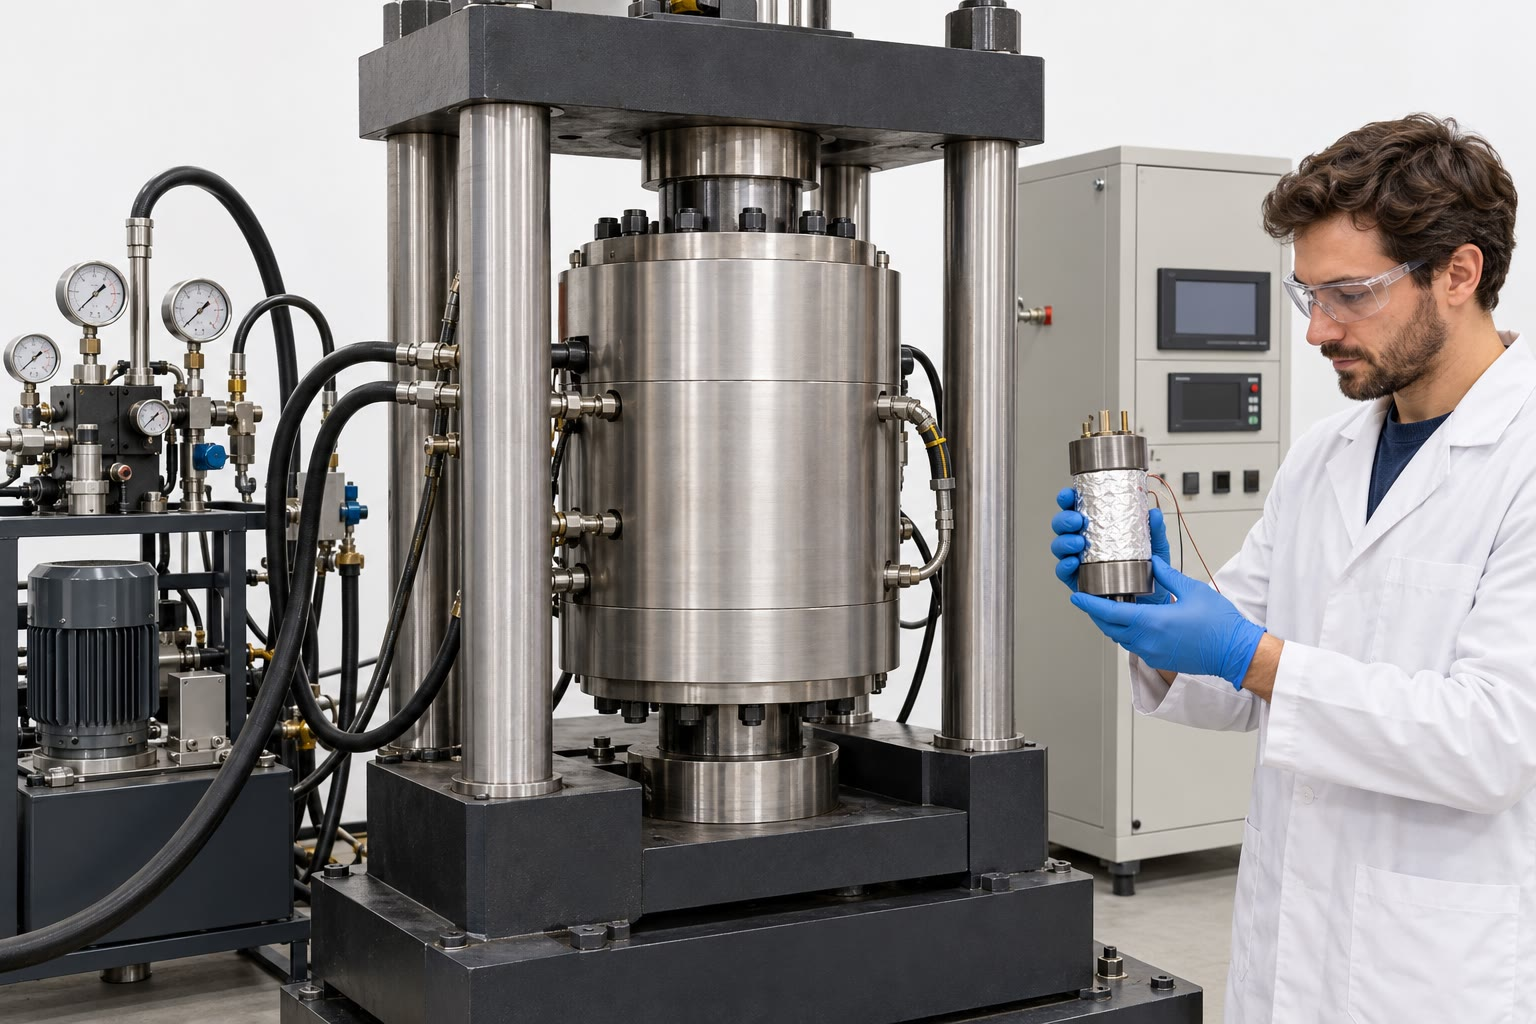
\includegraphics[width=\linewidth]{images/book5/ai/b3-deformation-press.jpg}

{\scriptsize جهاز ضغط لتشويه الصخور مع تجميعة عيّنة مغلّفة
(رسم توضيحي مولَّد بالذكاء الاصطناعي).}

\smallskip
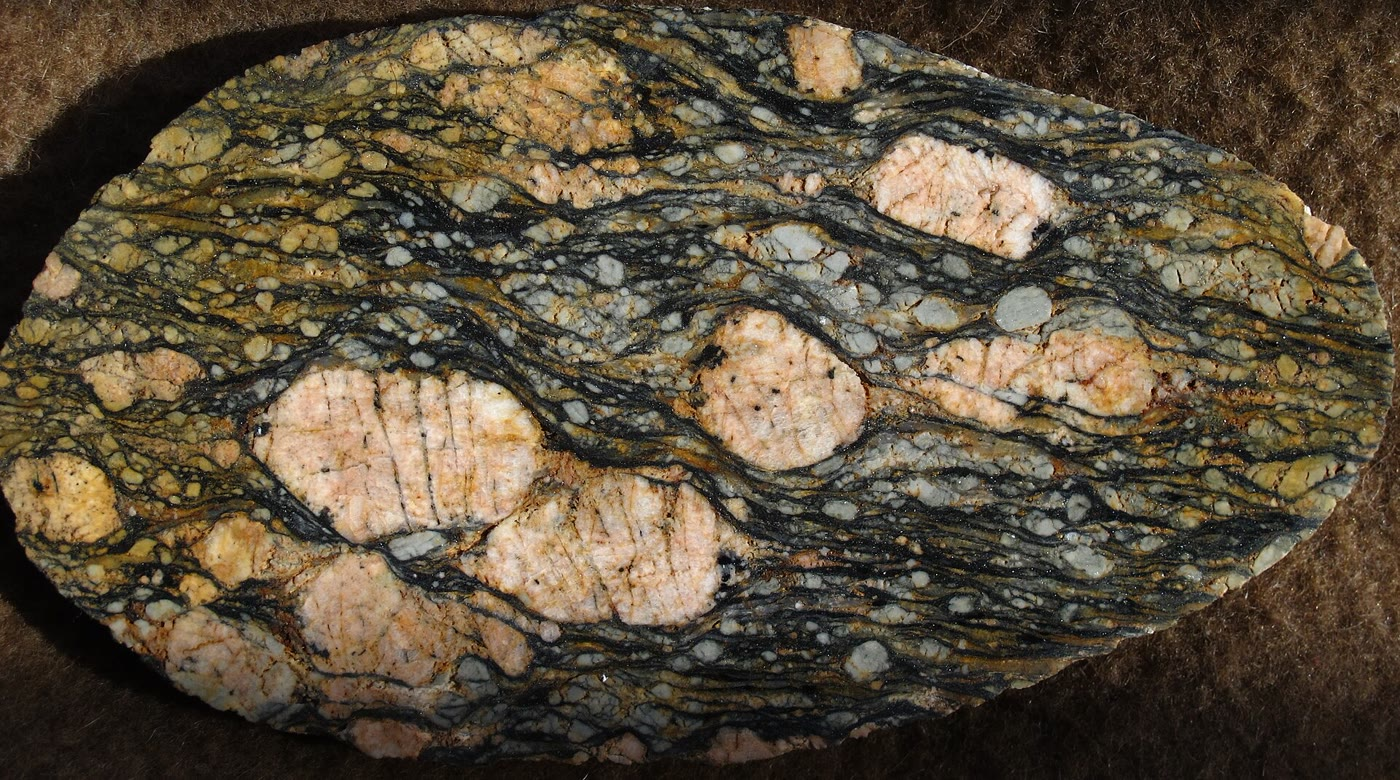
\includegraphics[width=\linewidth]{images/book5/b3-augen-mylonite.jpg}

{\scriptsize ميلونيت عيني مقطوع من النرويج: بورفيروكلاستات كبيرة من الفلسبار
في أرضية دقيقة من الكوارتز والفلسبار والميكا المعاد تبلورها. الصورة:
\mbox{\textdir TLT Mikenorton, CC BY-SA 4.0}.}
\end{minipage}
\end{inthelab}
% ledger: mk00:diffusion, photo:b3-augen-mylonite

\section{التمارين}

\begin{exercise}[$\star$]\label{exo:b3:deformation-mechanisms:1}
يذوب الفورستيريت عند \qty{1890}{\celsius} والجليد عند \qty{0}{\celsius}. احسب
\omterm{def:b3:deformation-mechanisms:flow-law}{درجة الحرارة المتجانسة} للفورستيريت عند \qty{1300}{\celsius} وللجليد عند
\qty{-10}{\celsius}. أيّهما يزحف بسهولة أكبر؟
\end{exercise}

\begin{exercise}[$\star$]\label{exo:b3:deformation-mechanisms:2}
ينحرف قاطعٌ يعبر نطاق قصّ عموديًا داخل النطاق بمقدار
\ang{70}، وينحرف قاطعٌ آخر بمقدار \ang{80}. احسب انفعالات القصّ. لماذا
يصعب قياس الانفعالات الكبيرة بهذه الطريقة؟
\end{exercise}

\begin{exercise}[$\star$]\label{exo:b3:deformation-mechanisms:3}
باستخدام \omterm{def:b3:deformation-mechanisms:piezometer}{مقياس الإجهاد القديم} للكوارتز، ما الإجهاد الذي يدلّ عليه
حجم حبيبات معادة التبلور \qty{10}{\micro m}؟
\end{exercise}

\begin{exercise}[$\star$]\label{exo:b3:deformation-mechanisms:4}
باستخدام \omterm{def:b3:deformation-mechanisms:flow-law}{قانون الانسياب} للكوارتزيت الرطب ($A = \num{1.1e-4}$، $n = 4$، $E =
\qty{223}{kJ.mol^{-1}}$)، $R = \qty{8.314}{J.mol^{-1}.K^{-1}}$)، احسب
معدّل الانفعال عند \qty{500}{\celsius} تحت \qty{20}{MPa}.
\end{exercise}

\begin{exercise}[$\star\star$]\label{exo:b3:deformation-mechanisms:5}
احسب اللزوجة الفعّالة للكوارتزيت الرطب المنساب بمعدّل انفعال \qty{e-14}{s^{-1}}
عند \qty{400}{\celsius} (\qty{65.4}{MPa}) وعند \qty{500}{\celsius}
(\qty{18.0}{MPa}). قارِن بلزوجات الوشاح
الواردة في \cref{ch:b3:mantle-convection}.
\end{exercise}

\begin{exercise}[$\star\star$]\label{exo:b3:deformation-mechanisms:6}
تُعطيان عند درجة الحرارة نفسها معدّل انفعال \qty{e-5}{s^{-1}} تحت
\qty{100}{MPa} و\qty{1.6e-4}{s^{-1}} تحت \qty{200}{MPa}. احسب \omterm{def:b3:deformation-mechanisms:flow-law}{أسّ الإجهاد}
وسمِّ الآلية المرجّحة.
\end{exercise}

\begin{exercise}[$\star\star$]\label{exo:b3:deformation-mechanisms:7}
عند الإجهاد نفسه، تزحف عيّنة أسرع عشر مرّات عند \qty{1100}{K} منها عند
\qty{1000}{K}. احسب طاقة التنشيط.
\end{exercise}

\begin{exercise}[$\star\star$]\label{exo:b3:deformation-mechanisms:8}
بأيّ عامل يتغيّر معدّل انفعال \omterm{def:b3:deformation-mechanisms:creep}{الزحف الانتشاري} عندما يُقسَم حجم الحبيبات
على عشرة، في حالتي زحف نابارو--هيرينغ وزحف كوبل؟ لماذا يكون زحف كوبل
أكثر حساسيةً؟
\end{exercise}

\begin{exercise}[$\star\star$]\label{exo:b3:deformation-mechanisms:9}
بالنسبة إلى الأوليفين الجاف عند \qty{1100}{\celsius} و\qty{2}{GPa}، يُعطي كلٌّ من قانوني الانسياب
$\dot\varepsilon_{\mathrm{dis}} = \num{6.54e-17}\,\sigma^{3.5}$
و$\dot\varepsilon_{\mathrm{dif}} = \num{3.59e-6}\,\sigma d^{-3}$ (بوحدات النصّ). احسب إجهاد الحدّ
من أجل $d = \qty{1}{mm}$ و$d =
\qty{100}{\micro m}$، وميل الحدّ.
\end{exercise}

\begin{exercise}[$\star\star\star$]\label{exo:b3:deformation-mechanisms:10}
حسب \cref{prop:b3:deformation-mechanisms:grain-size}،
فسّر لماذا يعطي المسار الشبكي $d^{-2}$ ومسار الحدود $d^{-3}$، وأظهِر
أنّ انتشار الحدود يتفوّق تحت حجم الحبيبات $d^* \approx
(B_B/B_L)\,\delta D_B/D_L$.
\end{exercise}

\begin{exercise}[$\star\star\star$]\label{exo:b3:deformation-mechanisms:11}
بالنسبة إلى قانون انسياب ذي $n = 3.5$، بأيّ عامل تنخفض اللزوجة الفعّالة
عند ضرب معدّل الانفعال بعشرة؟ لماذا يُرجِّح ذلك
تمركُزَ الانفعال في نطاقات القصّ؟
\end{exercise}

\begin{exercise}[$\star\star\star$]\label{exo:b3:deformation-mechanisms:12}
في الأوليفين الجاف الوارد في التمرين 9، يُعاد تبلور نطاق قصّ وشاحي تحت \qty{10}{MPa}
فتتحوّل حبيباته من \qty{3}{mm} إلى \qty{30}{\micro m}. احسب معدّل الانفعال الكلّي
قبل ذلك وبعده، وعامل التليين. أيّ آلية
تحمل التشوّه في كلّ حالة؟
\end{exercise}

\section{مسألة: نطاق القصّ في تلال فاردن}

\begin{problem}[{مسألة نهاية الأسبوع --- الانفعال والإجهاد ومعدّل الانفعال والعمر
لنطاق قصّ متخيَّل}]
\label{pb:b3:deformation-mechanisms:1}
% values: calc/ch07.py; flow_laws.py; st03:piezometer, lopez:flow-laws
تحت جرانيت تلال فاردن، المنطقة المُتخيَّلة للسلسلة، يكشف كلٌّ من ثقب الحفر
وقطع طريق عميق (كلاهما مُتخيَّل) نطاقَ قصّ لدنٍ عرضُه \qty{400}{m}،
تشكّل على عمق نحو \qty{15}{km} وعند \qty{450}{\celsius}.
يصنع قاطعُ دولريتٍ يعبر الجدران على زوايا قائمة، داخل النطاق،
زاويةً قدرها \ang{6} فقط مع حدود النطاق. كوارتزُه ميلونيتٌ من حبيبات معادة التبلور
عرض كلّ منها \qty{20}{\micro m} (تتراوح بين 15
و\qty{25}{\micro m}). خذ \omterm{def:b3:deformation-mechanisms:piezometer}{مقياس الإجهاد القديم} للكوارتز $D = 10^{3.56}\sigma^{-1.26}$،
وقانون انسياب الكوارتزيت الرطب ($A = \num{1.1e-4}$، $n = 4$، $E =
\qty{223}{kJ.mol^{-1}}$), $R = \qty{8.314}{J.mol^{-1}.K^{-1}}$, \qty{1}{yr} $=
\qty{3.156e7}{s}$، وفي القصّ البسيط، $\dot\gamma = 2\dot\varepsilon$.

\medskip\noindent\textbf{الجزء الأول --- الانفعال.}
\begin{enumerate}
  \item احسب انحراف القاطع $\psi$ وانفعال القصّ.
  \item احسب إزاحة أحد الجدارين بالنسبة إلى الآخر.
  \item احسب الاستطالات الرئيسية للقطع الناقص للانفعال ونسبته
        المحورية.
  \item احسب زاوية المحور الطويل مع النطاق. ماذا يفعل
        تورّق النطاق مع ازدياد $\gamma$؟
  \item عند النظر من الأعلى، يتتبَّع القاطع من الجدار الجنوبي فينعطف نحو الشرق
        عند دخوله نطاق الشرق--غرب، ثم يعود إلى اتجاهه نحو الشمال عند الجدار الشمالي.
        في أيّ اتجاه تحرّك الجدار الشمالي،
        وهل النطاق أيمن أم أيسر؟
  \item في أيّ مستوى ينبغي أن تُقطَع شريحة رقيقة لقراءة المؤشّرات الحركية،
        وكيف ينبغي أن يميل تورّق S فيها؟
\end{enumerate}

\medskip\noindent\textbf{الجزء الثاني --- الإجهاد.}
\begin{enumerate}[resume]
  \item احسب الإجهاد الذي تدلّ عليه الحبيبات البالغ عرضها \qty{20}{\micro m}.
  \item احسب الإجهادين عند 15 و\qty{25}{\micro m}.
  \item هل يقع الإجهاد ضمن مدى المعايرة؟
  \item لم يُظهر \omterm{def:b3:deformation-mechanisms:piezometer}{مقياس الإجهاد القديم} أيّ أثر لدرجة الحرارة. لماذا يهمّ ذلك
        هنا؟
  \item ما حجم الحبيبات الذي كان سيُنتجه إجهاد قدره \qty{100}{MPa}؟
\end{enumerate}

\medskip\noindent\textbf{الجزء الثالث --- معدّل الانفعال.}
\begin{enumerate}[resume]
  \item احسب $E/RT$ عند \qty{450}{\celsius} وعامل أرهينيوس.
  \item احسب معدّل انفعال الكوارتز تحت الإجهاد الوارد في السؤال 7
        (خذ \qty{62}{MPa}).
  \item احسب معدّل انفعال القصّ.
  \item احسب اللزوجة الفعّالة للنطاق وقارنها بالوشاح العلوي
        من \cref{ch:b3:mantle-convection}.
  \item بأيّ عوامل يتغيّر معدّل الانفعال عند 400
        و\qty{500}{\celsius} عند الإجهاد نفسه؟
  \item بأيّ عامل يتغيّر المعدّل لو كان الإجهاد \qty{78}{MPa} المقابل
        لأدقّ الحبيبات؟
\end{enumerate}

\medskip\noindent\textbf{الجزء الرابع --- الزمن.}
\begin{enumerate}[resume]
  \item احسب الزمن اللازم لتراكم انفعال القصّ الوارد في السؤال 1،
        بالثواني.
  \item حوّله إلى آلاف السنين.
  \item احسب متوسط معدّل الانزلاق عبر النطاق بوحدة \unit{mm/yr}.
  \item قارنه بمعدّلات حدود الصفائح التي تبلغ عشرات المليمترات في السنة.
        % ledger: morvel:range
  \item لو كان النطاق يحمل \qty{20}{mm/yr}، فما معدّل انفعال القصّ والإجهاد
        وحجم الحبيبات المعادة التبلور الذي كان سيكون عليه؟
  \item كيف تؤثّر حالات عدم اليقين في حجم الحبيبات وفي أسّ \omterm{def:b3:deformation-mechanisms:piezometer}{مقياس الإجهاد القديم}
        على الزمن؟
  \item أعطِ الزمن الذي استغرقه \omterm{def:b3:deformation-mechanisms:shear-zone}{نطاق القصّ} في تلال فاردن لتراكم انفعاله، بآلاف
        السنين.
\end{enumerate}
\end{problem}
